\documentclass[portuguese,oneside]{tcc}

\usepackage{graphicx}
\usepackage{multirow}
\usepackage{nicefrac}
\usepackage{algorithmic}
\usepackage{calc}
\usepackage{enumitem}
\usepackage{tikz}
\usepackage{pgfgantt}
\usepackage{mdframed}

\usepackage{listings}
\lstdefinestyle{customC++}{
	frame=single,
	language=c++,
	numbers=left,
	numbersep=5pt,
	tabsize=2,
	basicstyle=\footnotesize
}

\usepackage{subcaption}
\captionsetup{compatibility=false}

\usetikzlibrary{shapes.geometric}
\usetikzlibrary{shapes.misc}
\usetikzlibrary{positioning}
\usetikzlibrary{fit}
\usetikzlibrary{trees}

\author{Martin Duarte Móre e William Henrihque Martins}

\title{Explorando as Cavernas de Spelunky Utilizando Agentes Inteligentes}
      {Exploring Spelunky's Caves Using Intelligent Agents}

\tipotrabalho{\tci}

\curso{\cc}

\orientador{Felipe Meneguzzi}

\begin{document}

%\dedicatoria{Dedico este trabalho a meus pais.}

%\epigrafe{The art of simplicity is a puzzle of complexity.}
%         {Douglas Horton}

%\begin{agradecimentos}
%\end{agradecimentos}

\begin{resumo}{Spelunky, jogo de computador, SpelunkBots, inteligência
artificial, agentes inteligentes}
\textit{Spelunky} é um premiado jogo de computador fácil de aprender, mas
difícil de dominar. O objetivo do jogador é explorar cavernas subterrâneas
enquanto coleta tesouros valiosos e evita monstros e armadilhas. Este trabalho
tem como objetivo desenvolver soluções de Inteligência Artificial para a criação
de agentes inteligentes capazes de jogar com autonomia o jogo \textit{Spelunky}.
\end{resumo}

\begin{abstract}{Spelunky, computer game, SpelunkBots, artificial intelligence,
intelligent agents}
\textit{Spelunky} is an award-winning computer game that is easy to learn, but
hard to master. The player's goal is to explore underground caves whilst
collecting valuable treasures and avoiding monsters and traps. This work aims to
develop Artificial Intelligence solutions for creating intelligent agents
capable of playing autonomously the game \textit{Spelunky}.
\end{abstract}

\listoffigures
%\listoftables
\listofalgorithms
\listofacronyms
%\listofabbreviations
%\listofsymbols
\tableofcontents

\chapter{\label{chap:introduction}Introdução}

\sigla{API}{Application Programming Interface}
\sigla{BT}{Behavior Tree}
\sigla{DLL}{Dynamic-link Library}
\sigla{FSM}{Finite-State Machine}
\sigla{GML}{GameMaker Language}
\sigla{HFSM}{Hierarchical Finite-State Machine}
\sigla{NEAT}{Neuroevolution of Augmenting Topologies}
\sigla{TWEANN}{Topology and Weight Evolving Artificial Neural Network}

A popularização dos jogos digitais se deu nas décadas de 70 e 80 com o
surgimento dos computadores pessoais, os fliperamas e os \textit{consoles} de
jogos. Apesar de sofrer uma retração com o \textit{crash} de
83\footnote{Recessão na indústria de jogos digitais que ocorreu de 1983 a 1985.
A principal causa foi a saturação do mercado.}, o mercado de jogos digitais
ascendeu rapidamente. Em 2014, obteve uma receita de aproximadamente 80 bilhões
de
dólares\footnote{https://newzoo.com/insights/articles/top-100-countries-represent-99-6-81-5bn-global-games-market/}.
Isto mostra que os seres humanos possuem um interesse significativo por jogos
digitais. Como consequência, a indústria está em constante aprimoramento,
buscando produzir jogos mais interessantes, inovadores e desafiadores, a fim de
manter seu público alvo e atrair novos jogadores. Um dos aliados dos jogos
digitais para atingir este objetivo é o uso de técnicas sofisticadas de
inteligência artificial para criar conteúdos complexos e engajar ainda mais
os jogadores\cite{PanoramaAIGames}.

Paralelamente, a área de inteligência artificial também se beneficia ao se
relacionar com jogos digitais. Jogos podem ser utilizados como plataformas de
testes para seus algoritmos e técnicas, pois são muito acessíveis, são capazes
de reproduzir cenários reais em ambientes virtuais e seu uso torna o processo
mais barato e rápido que, por exemplo, realizar testes no mundo real com objetos
físicos\footnote{http://togelius.blogspot.com/2016/01/why-videogames-are-essential-for.html}.
Diversas competições de inteligência artificial foram criadas recentemente
utilizando jogos digitais como plataforma de teste\cite{GameAiCompetition}.
Estas competições geralmente possuem como objetivo principal a criação de
agentes inteligentes capazes de jogar o jogo proposto da maneira mais eficiente
possível, seja por pontuação, seja por tempo. Uma destas competições, baseada no
jogo de computador \textit{Spelunky}, se chama \textit{SpelunkBots}. Os
criadores desta competição desenvolveram uma aplicação de inteligência
artificial que facilita a criação de agentes inteligentes para o jogo.

\textit{Spelunky} é um jogo de computador considerado fácil de aprender mas
extremamente difícil de dominar, pois requer que o jogador possua reações
rápidas para perigos iminentes e, ao mesmo tempo, pense em táticas e estratégias
de longo prazo para ser bem-sucedido. Ao todo, são 26 inimigos, 14 armadilhas e
43 itens diferentes\footnote{Dados extraídos da Spelunky Wiki
(http://spelunky.wikia.com/wiki/Spelunky\_Wiki).}. O jogador, ao iniciar uma
partida, sempre se depara com um nível completamente diferente, pois o jogo faz
uso de um algoritmo complexo para gerar níveis. Estes fatores fazem com que
\textit{Spelunky} seja um jogo com desafios interessantes para a pesquisa em
inteligência artificial.

Este trabalho tem como objetivo a construção de agentes inteligentes capazes de
jogar o jogo \textit{Spelunky}, considerado como um problema de difícil solução
\cite{SPELUNKYHARD}.  Para tal, utilizaremos o \textit{framework}
\textit{SpelunkBots} e implementaremos as técnicas de inteligência artificial
\textit{Behavior Trees} e \textit{NEAT} em agentes jogadores de
\textit{Spelunky}, avaliando e comparando seus desempenhos e resultados obtidos.

\todo{Não usamos mais Behavior Trees}

Primeiramente, no capítulo \ref{chap:introduction}, apresentamos uma breve
contextualização da relação entre jogos digitais e inteligência artificial,
nossas motivações para o surgimento deste projeto, uma descrição resumida de
nossos objetivos e um detalhamento da estrutura deste documento. Depois, no
capítulo \ref{chap:spelunky}, examinamos o universo do jogo \textit{Spelunky}.
Em seguida, no capítulo \ref{chap:spelunkbots}, levantaremos alguns pontos
importantes sobre competições de inteligência artificial com base em jogos
digitais e, depois disso, forneceremos uma breve explicação do funcionamento do
\textit{framework} \textit{SpelunkBots}. No capítulo \ref{chap:theory},
estabelecemos a base teórica necessária para compreender as técnicas de
inteligência artificial escolhidas para o desenvolvimento dos \textit{bots}.
Depois, no capítulo \ref{chap:project}, apresentamos uma explicação dos
problemas e objetivos deste trabalho, e depois traçamos os requisitos e detalhes
do projeto de implementação. Por fim, no capítulo \ref{chap:work-plan},
definimos as atividaddes necessárias para atingirmos os objetivos estipulados e
apresentamos um cronograma de execução deste projeto.

\todo{Não usamos mais um capítulo de planejamento}

\chapter{\label{chap:spelunky}Spelunky}
Spelunky\footnote{http://www.spelunkyworld.com/original.html} é um jogo onde o
jogador incorpora um aventureiro que decide explorar uma caverna misteriosa. O
local contém tesouros, mas também está repleto de perigos. O objetivo principal
do jogador é explorar estas cavernas subterrâneas e coletar a maior quantia de
tesouros possível enquanto evita ser abatido pelos diversos inimigos e
armadilhas espalhadas pelo ambiente. A Figura \ref{fig:spelunky-gameplay}
ilustra uma partida do jogo.

\begin{figure}[htb!]
\centering
\includegraphics[width=.65\textwidth]{fig/spelunky-pc-screen.png}
\caption{\label{fig:spelunky-gameplay}Exemplo de partida de spelunky, mostrando
elementos do jogo como o jogador, a caverna, os inimigos, os tesouros, entre
outros.}
\end{figure}

O jogo se enquadra no gênero \textit{platformer}, estilo de jogo que envolve
guiar um personagem através de plataformas suspensas e obstáculos para obter
progresso no jogo. Também faz uso de alguns dos elementos-chave do gênero
\textit{roguelike} -- tipo de jogos que se popularizou na década de 80
caracterizados por sua dificuldade, enfoque em exploração de ambientes e
narrativa fantasiosa --, como \textbf{geração procedural} e \textbf{morte
permanente}. Os níveis de Spelunky são gerados proceduralmente, ou seja, utiliza
um algoritmo capaz de gerar automáticamente os elementos que irão compor o
nível. Isto significa que não existe uma maneira de se memorizar estratégias
específicas de um mapa em Spelunky, pois ao início de cada partida o mapa é
gerado de maneira única e os tesouros, itens e obstáculos são dispostos de
maneira diferente, fazendo com que o jogador tenha que aprender a lidar com os
elementos do jogo de forma individual, combinar este conhecimento e estabelecer
uma estratégia para vencer seus obstáculos e ser bem sucedido. A seção
\ref{section:spelunky-procgen} explica em maiores detalhes o algoritmo utilizado
para geração procedural. Além disso, o jogo conta com o conceito de morte
permanente, que faz com que o jogador, ao ter seus pontos de vida esgotados,
tenha que recomeçar o jogo desde seu início, perdendo todo o progresso obtido
até então.

\section{\label{section:spelunky-goals}Objetivos}
Spelunky é um jogo que baseia a qualidade das partidas utilizando um sistema de
\textit{high scores}. Para tal, faz uso de uma série de métricas para
classificar os jogadores ao término de uma partida. Estas métricas são:
\textbf{quantidade de tesouros}, \textbf{número de abates}, \textbf{número de
donzelas salvas} e \textbf{tempo total de partida}. A Figura
\ref{fig:spelunky-scores} mostra um exemplo de pontuação final obtida.

\begin{figure}[htb!]
\centering
\includegraphics[width=.65\textwidth]{fig/spelunky-score.png}
\caption{\label{fig:spelunky-scores}Exemplo de pontuação final obtida ao fim de
uma partida de Spelunky.}
\end{figure}

Apesar de oferecer 4 pontuações diferentes, a comunidade de jogadores de
Spelunky não mostra interesse significativo em atingir quantidades elevadas de
número de abates e número de donzelas salvas, se concentrando em atingir
pontuações máximas em número de tesouros e em concluir o jogo no menor tempo
possível\footnote{Comunidade de ranking de jogadores de Spelunky:
https://mosstier.com}. Pode-se concluir, portanto, que o \textbf{objetivo
principal} é chegar ao fim do jogo e os \textbf{objetivos secundários} mais
importantes são a pontuação final e o tempo total da partida.

\section{\label{section:spelunky-structure}Estrutura do jogo}
% nivel
% area
% partida

\section{\label{section:spelunky-controls}Controle do Personagem}
% possiveis acoes que o jogador pode executar

\section{\label{section:spelunky-procgen}Algoritmo de Geração Procedural de
Níveis}
% entrar em detalhes

\section{\label{section:spelunky-obstacles}Obstáculos}
% inimigos (listar)
% armadilhas (listar)
% ambiente (quedas, lava, etc.)

\section{\label{section:spelunky-items}Itens}
% três categorias diferentes: consumíveis, acessórios e armas
% listar todos e dar breve explicação

\section{\label{section:spelunky-dev}Desenvolvimento e Distribuição}
O jogo foi desenvolvido por Derek Yu -- utilizando o motor de desenvolvimento de
jogos \textit{GameMaker} (Versão 8.0 Pro) -- e lançado gratuitamente para a
plataforma \textit{Windows} em dezembro de
2008\footnote{https://forums.tigsource.com/index.php?topic=4017}. No fim de
2009, o criador optou por liberar o código fonte do jogo, permitindo sua
distribuição não-comercial e
modificação\footnote{http://www.spelunkyworld.com/files/COPYING.txt}. A
liberação do código fonte de Spelunky pode ser considerada um marco muito
importante, pois permitiu que fossem criadas modificações para o jogo. Estas
modificações, que podem ser encontradas no fórum oficial da
\textit{Mossmouth}\footnote{http://mossmouth.com/forums/index.php} -- empresa
desenvolvedora de jogos criada por Derek Yu --, são correções de \textit{bugs},
mapas customizados ou até mesmo modos de jogo completamente diferentes do jogo
original. Pode-se dizer que dar esta liberdade para a comunidade do jogo é um
dos fatores que ajuda a manter sua base de jogadores e atraem novos jogadores
até hoje.

O motor GameMaker disponibiliza diversas ferramentas que facilitam o trabalho
do desenvolvedor. Contando com funcionalidades como editores de
\textit{scripts}\footnote{Código desenvolvido para o controle dos
comportamentos dos elementos do jogo.} e de \textit{sprites}\footnote{Elementos
visuais do jogo, tais como o personagem, o fundo, os inimigos. Representados
como uma ou mais imagens, permitindo que as mesmas sejam animadas.},
gerenciadores de eventos, entre
outras\footnote{http://sandbox.yoyogames.com/downloads/docs/gmaker80.pdf}, o
GameMaker oferece um ótimo suporte ao desenvolvedor para a criação de jogos. O
motor disponibiliza uma linguagem de programação própria para seus
\textit{scripts}, a \textit{GameMaker Language}, ou \textit{GML}.

\chapter{\label{chap:spelunkbots}SpelunkBots}

Utilizando o código-fonte de Spelunky, Daniel Scales e Thomas Thompson, da
Universidade de Derby no Reino Unido, criaram o
\textit{SpelunkBots}\cite{SPELUNKBOTSPAPER}, um
\textit{framework} que permite a programação de \textit{bots} para o jogo
Spelunky. Um dos objetivos dos criadores é utilizar a aplicação para criar uma
competição de inteligência artificial para o jogo.

A \textit{API} possibilita que o desenvolvedor resgate informações de objetos
estáticos e dinâmicos contidos no ambiente do jogo, como o terreno, a
posição de tesouros, armadilhas e inimigos. Contudo, o objetivo da \textit{API}
disponibilizada por SpelunkBots é fazer com que a informação recebida pelo
\textit{bot} se assemelhe ao máximo com a percepção de um jogador humano.  Para
tal, o \textit{framework} implementa um sistema de \textit{fog of war},
limitando o conhecimento do ambiente que pode ser obtido pela inteligência
artificial. Para objetos estáticos, uma vez que o jogador visualizou o objeto,
ele poderá receber informações sobre ele permanentemente. Para objetos
dinâmicos, o \textit{bot} só poderá receber informações sobre eles se os mesmos
estiverem sendo visualizados por ele. A figura \ref{fig:spelunkbots-fow} ilustra
um exemplo de funcionamento do sistema, onde as áreas apresentadas na coloração
cinza e marcadas com o valor ``1'' representam pontos sobre os quais o
\textit{bot} não tem conhecimento algum, pois ainda não explorou a área
que o permite que sejam revelados os elementos do jogo que se encontram
nesses pontos.

\begin{figure}[htb!]
\centering
\includegraphics[width=.65\textwidth]{fig/spelunkbots-fow.png}
\caption {\label{fig:spelunkbots-fow}Visualização do sistema de \textit{fog of
war} demonstrando a diferença de informação recebida de elementos dentro e fora
do campo de visão do jogador.}
\end{figure}

\section{Utilização da \textit{API}}

É possível desenvolver \textit{bots} que fazem uso da \textit{API}
utilizando a linguagem GML (sigla para \textit{Game Maker Language}) ou
através da linguagem C++, ficando a critério do desenvolvedor a escolha da
linguagem. A única restrição que existe quanto ao uso de C++ dá-se no fato
de que a linguagem necessita de um processo de compilação através de uma
ferramenta externa, não sendo gerenciada diretamente pelo \textit{Game
Maker}. (COLOCAR FIGURINHA AQUI)

A \textit{API} permite uma interação completa com o jogo através do uso
das variáveis expostas pelo
\textit{framework}\footnote{http://spelunkbots.com/wp-content/uploads/2015/02/SpelunkBots-API-A-Getting-Started-Tutorial.pdf}.
Com essas variáveis é possível fazer o controle da movimentação do bot, bem
como identificar o tipo de terreno em que se está pisando e os inimigos que
aparecem em seu campo de visão. Além disso, também são disponibilizadas
informações sobre as armadilhas que podem atrapalhar o jogador. Por fim,
existem variáveis que permitem um melhor controle das informações relativas ao
\textit{bot}, como o posicionamento no eixo X e no eixo Y, se o \textit{bot}
encontra-se virado para a esquerda ou para a direita, entre outros.

\begin{itemize}
    \item Motivação: citar os porquês de ter sido criado (citar o paper do
        Scales e do Thompson \cite{SPELUNKBOTSPAPER}), bem como as possíveis
        competições que surgem a partir da criação desses (só citar mesmo,
        entrar em detalhes no capítulo específico).
    \item Explicar sobre a API e suas características ``interessantes''
        (\textit{fog war} com figura e explicações)
    \item Explicar como é feito o uso da API por um desenvolvedor (GML ou
        C++). Talvez seja interessante explicar alguma coisa das DLLs,
        para o caso de usar C++ (aqui vai uma figurinha bacana mostrando a
        ``arquitetura'')
    \item Interação com o Jogo
        \footnote{http://spelunkbots.com/wp-content/uploads/2015/02/SpelunkBots-API-A-Getting-Started-Tutorial.pdf}
    \begin{itemize}
        \item Explicar as variáveis globais de movimentação
        \item Explicar as variáveis globais do terreno (talvez vale
            colocar figuras aqui)
        \item Explicar as variáveis globais dos obstáculos (inimigos vêm aqui)
        \item Explicar as variáveis globais referentes aos objetos
        \item Explicar as variáveis globais referentes ao player
    \end{itemize}
\end{itemize}

\chapter{\label{chap:theory}Fundamentação Teórica}
Neste capítulo, apresentaremos a base teórica necessária para compreender o
funcionamento das técnicas de inteligência artificial escolhidas para realizar o
desenvolvimento dos agentes inteligentes de \textit{Spelunky}.


%----------
\section{\label{section:environment}Ambientes}
Todas as percepções e ações executadas por agentes racionais ocorrem no
\textbf{ambiente} no qual ele está inserido. A quantidade e variedade de
ambientes encontrados é vasta, mas é possível identificar dimensões (ou
características) de classificação para realizar uma categorização destes
ambientes. Estas características irão determinar que tipos de agentes --
enumerados na seção \ref{section:agents} -- são apropriados para cada ambiente.
As dimensões utilizadas para categorizar ambientes são:

\begin{description}
	\item[Observável, Parcialmente Observável ou Não-Observável]
		Um ambiente é observável se os sensores do agente lhe permitirem acesso
		completo ao estado do ambiente a cada ponto no tempo. Ambientes
		observáveis são convenientes, pois o agente não precisa manter um estado
		interno de conhecimento para se manter informado. O ambiente é
		parcialmente observável se os sensores do agente possuirem ruído ou não
		tiverem acesso completo ao ambiente. Se o agente não possuir nenhum tipo
		de sensor, então o ambiente é não-observável.

	\item[Agente Único ou Multi-Agente]
		Quando o agente não precisa interagir com nenhum outro agente no
		ambiente, então trata-se de um ambiente com agente único. Caso ele
		precise interagir de alguma forma (competição, cooperação ou
		comunicação) com outros agentes, então o ambiente é multi-agente.

	\item[Determinístico ou Estocástico]
		Se o próximo estado do ambiente for completamente determinado pela
		combinação do estado atual com uma ação executada pelo agente, então o
		ambiente é determinístico. Caso contrário, é estocástico.

	\item[Episódico ou Sequencial]
		Em ambientes episódicos, a experiência do agente é dividida em episódios
		atômicos, ou seja, são independentes entre sí. O agente não precisa
		pensar adiante pois, a cada episódio, recebe informações sensoriais e
		executa apenas uma ação, e o próximo episódio não será influenciado pela
		ação anterior. Já em ambientes sequenciais, a ação atual pode
		influenciar todas as decisões futuras, ou seja, ações a curto prazo
		podem ter consequências a longo prazo.

	\item[Discreto ou Contínuo]
		Ambientes discretos são aqueles onde se tem um número contável de ações
		e percepções possíveis. Em ambientes contínuos, o número de ações e de
		percepções muitas vezes são baseados em valores contínuos ou não são
		contáveis.

	\item[Conhecido ou Desconhecido]
		Esta distinção não se refere ao ambiente em sí, e sim sobre o
		conhecimento do agente (ou criador do agente) das "leis" de
		comportamento do ambiente. Em um ambiente conhecido, os resultados (ou
		probabilidades de resultados) das ações são conhecidos. Quando o
		ambiente é desconhecido, o agente precisa primeiro aprender como o
		ambiente funciona para saber fazer escolhas boas para atingir seus
		objetivos.
\end{description}


%----------
\section{\label{section:agents}Agentes Racionais}
Um agente é uma entidade que utiliza seus \textbf{sensores} para perceber o
ambiente no qual está inserido e interage através de seus \textbf{atuadores},
direcionando seus esforços para alcançar algum objetivo que se propõe a
atingir\cite[cap. 2]{RussellNorvig200912}. Um exemplo de agente racional é o ser
humano, que percebe o ambiente através de seus sentidos (visão, audição, entre
outros) e executa ações com seu corpo (braços, pernas, etc.). De acordo com
Russell \& Norvig\cite{RussellNorvig200912}, agentes racionais são agrupados nas
seguintes categorias: \textbf{agentes reflexivos}, \textbf{agentes baseados em
modelo}, \textbf{agentes baseados em objetivos} e \textbf{agentes baseados em
utilidade}.

Os \textbf{agentes reflexivos} são programados para executar ações baseadas em
algum evento percebido. Fica evidente que este tipo de agente simplesmente
executa uma ação baseado em suas percepções imediatas e não guardam informações
sobre suas experiências passadas, sendo apenas reativos.

Diferentemente dos agentes reflexivos, \textbf{agentes baseados em modelo} são
capazes de guardar informações sobre suas experiências passadas e sobre seu
estado atual. Este tipo de agente compreende como suas ações modificam o
ambiente onde está inserido e como o ambiente se altera independentemente de
suas ações, efetivamente construíndo um \textbf{modelo} do ambiente. 

Às vezes, ter conhecimento sobre o estado atual do ambiente não é suficiente
para decidir que ação executar. O agente precisa de alguma informação de que
situações são desejáveis, ou que objetivos desejar cumprir. Este é o caso de
\textbf{agentes baseados em objetivo}, que combinam um modelo do ambiente com
informações de objetivo para escolher as ações que mais o aproximam dos estados
desejáveis. A escolha de ações baseada em objetivos pode ser simples -- quando,
por exemplo, o objetivo é antigido com a execução de apenas uma ação -- ou
complexo -- quando, por exemplo, o agente deve considerar longas cadeias de
ações para atingir seus objetivos.

Em alguns casos, os objetivos não são suficientes para gerar comportamentos de
alta qualidade. Por exemplo, muitas vezes é possível atingir um objetivo através
de várias sequências de ações, mas algumas sequências são mais rápidas, mais
seguras, mais confiáveis ou mais baratas. Os \textbf{agentes baseados em
utilidade} fazem uso de uma função de utilidade para medir sua performance e,
assim, distinguir estados mais desejáveis e menos desejáveis. O agente, então, é
capaz de escolher as ações mais vantajosas para ele, aumentando sua performance.


%----------
\section{\label{section:machine-learning}Aprendizado de Máquina}
Quando queremos resolver um problema através de um programa de computador,
desenvolvemos um algoritmo que, dado uma entrada, executa uma sequência de
operações para fornecer uma resposta adequada para a tarefa em questão. Um
exemplo disso seriam os algoritmos para ordenação de números, onde a entrada é
um conjunto de números e a resposta é o conjunto ordenado. Para alguns
problemas, contudo, nem sempre é possível se chegar a um algoritmo que resolve
satisfatóriamente uma tarefa. Por exemplo, a tarefa de diferenciar
\textit{e-mails} de \textit{spam} e \textit{e-mails} legítimos é complexa, pois
os \textit{e-mails} de \textit{spam} estão mudando constantemente, e a
categorização de \textit{spam} pode variar de indivíduo para indivíduo. Assim,
criar manualmente um algoritmo para resolver esta tarefa pode ser extremamente
complexo ou até mesmo impraticável. A partir deste contexto, surgiu a área de
\textbf{aprendizado de máquina}, que estuda algoritmos que fornecem a programas
de computador a habilidade de aprender e se aperfeiçoarem, tornando-os capazes
de resolver tarefas sem serem explicitamente programados.

Existem três tipos principais de aprendizado de máquina\cite[cap.
18]{RussellNorvig200912}, que são diferenciados entre sí pelo tipo de
\textit{feedback} retornado pelo problema. Estas categorias são:
\textbf{aprendizado supervisionado}, \textbf{aprendizado não-supervisionado} e
\textbf{aprendizado por reforço}. No aprendizado supervisionado, é fornecido um
conjunto de dados com exemplos de entrada e resultados esperados para aquelas
entradas. Assim, a tarefa neste tipo de aprendizado consiste em aprender uma
função que mapeia entradas para saídas. No aprendizado não-supervisionado, o
programa recebe um conjunto de dados de entrada mas não recebe informações com o
tipo de saída esperado. O objetivo deste tipo de aprendizado geralmente é
detectar padrões em conjuntos de dados.  O último tipo de aprendizado, o
aprendizado por reforço, é diferente dos demais porque está diretamente ligado
ao conceito de agentes racionais.  Neste tipo de aprendizado, o agente interage
com um ambiente dinâmico e deve atingir algum objetivo. Quando o agente executa
ações no ambiente, é fornecido a ele algum tipo de retorno -- recompensas ou
punições --, para que ele possa aprender a agir da maneira correta a fim de
atingir seus objetivos.

Para agentes racionais, a capacidade de aprender fornece a oportunidade de se
tornar mais competente que o permitido pelo seu conhecimento inicial do problema
e do ambiente. Problemas como informação incompleta ou inexistente sobre o
ambiente são mais facilmente contornados, pois o agente será capaz de criar um
modelo de representação através do retorno obtido após a execução de ações.


%----------
\section{\label{section:neural-networks}Redes Neurais Artificiais}
Uma \textbf{rede neural artificial} é um modelo matemático que busca replicar
computacionalmente (através de aproximações de funções) as capacidades de
processamento de informações de sistemas nervosos
biológicos\cite{Rojas:1996:NNS:235222}. Recentemente, redes neurais artificiais
vem recebendo uma atenção especial, mas esta técnica teve suas origens no início
da década de 40\cite{RussellNorvig200912}. Esta seção apresenta apenas um resumo
geral de redes neurais artificiais, pois o assunto é muito complexo e um
entendimento superficial do funcionamento desta técnica é suficiente para este
trabalho.

Os elementos mais primitivos das redes neurais são as unidades de processamento
chamadas \textbf{neurônios} -- ilustrado na Figura
\ref{fig:neural-networks-neurons}.  Cada neurônio possui canais de
\textbf{entrada} através dos quais recebe as informações que deverá processar.
Cada canal de entrada possui um \textbf{peso}, que informa ao neurônio o quão
relevante a informação advinda daquela conexão é importante. Com estas
informações em mãos, realiza um processamento interno através de sua
\textbf{função de ativação}. Depois, envia a informação processada adiante, ou
para mais processamento em neurônios adicionais, ou como resultado final da
operação.

Para processar as informações do problema (e, assim, gerar uma função da rede),
as redes neurais organizam as conexões e localizações de seus neurônios de uma
maneira específica, formando uma \textbf{topologia} da rede. Basicamente, 

\begin{figure}[H]
\centering
\caption {\label{fig:neural-networks-neuron}Ilustração que indica os principais
componentes de um neurônio de uma rede neural artificial.}
\end{figure}


\begin{mdframed}[backgroundcolor=green!20]
\begin{itemize}
	\item
		Explicar
\end{itemize}
\end{mdframed}



%----------
\section{\label{section:environment}Algoritmos Evolutivos}
\begin{mdframed}[backgroundcolor=green!20]
\begin{itemize}
	\item
		Explicar
\end{itemize}
\end{mdframed}



%----------
\section{\label{section:behavior-trees}Behavior Trees}
A construção de bons agentes inteligentes depende fortemente da capacidade que
os agentes têm de tomar boas decisões de comportamento. No contexto de jogos
digitais, a partir da década de 90, a qualidade da inteligência artificial
passou a ser um diferencial no momento de compra de um jogo\cite[Cap.
1]{Millington:2009:AIG:1795711}, aumentando a importância da escolha de uma
técnica apropriada para desenvolver os agentes inteligentes.Das técnicas mais
populares, a \textbf{\textit{Behavior Tree}}, ou Árvore de Comportamento, é uma
das técnicas que mais se destaca, devido a sua \textbf{simplicidade} e
\textbf{extensibilidade}\cite[Cap.  4]{Rabin:2013:GAP:2566761}, e já foi
utilizada na indústria em jogos como \textit{Halo 2}\cite[Cap.
5]{Millington:2009:AIG:1795711} e
\textit{Spore}\footnote{http://chrishecker.com/My\_liner\_notes\_for\_spore},
por exemplo.

Uma \textit{Behavior Tree} é uma estrutura de dados baseada em árvore que contém
um nodo \textbf{raíz} (geralmente utilizada para controlar o fluxo inicial de
execução) e vários nodos filhos que representam os \textbf{comportamentos}. Cada
comportamento deve possuir uma \textbf{pré-condição} e uma \textbf{ação}. Caso a
pré-condição seja satisfeita, o agente poderá executar o comportamento descrito
pela ação do nodo\cite[Cap. 4]{Rabin:2013:GAP:2566761}. Isto faz com que o
algoritmo de execução seja simples: partimos do nodo raíz em busca do primeiro
filho que satisfaça sua pré-condição (geralmente da esquerda para a direita). Ao
encontrá-lo, executamos sua ação. É importante ressaltar que somente um
comportamento é selecionado por vez. Portanto, se um comportamento for
selecionado, o algoritmo não tentará executar as ações dos nodos vizinhos na
mesma execução do algoritmo.

É possível adicionar estruturas de \textbf{controle de fluxo} a uma
\textit{Behavior Tree}. Desta forma, os ramos da árvore passam a ser usados para
controlar o fluxo de execução, enquanto os nodos-folha representam as
pré-condições e ações\cite[Cap. 10]{Rabin:2015:GAP:2821138}. Quando uma ação de
um nodo-folha é executado, ele informa ao seu pai (controlador de fluxo) o
estado de sua execução -- sucesso, falha ou em andamento. Existem diversos
tipos de estruturas de controle de fluxo que são utilizadas em \textit{Behavior
Trees}, mas as mais comuns são os de \textbf{seleção} e de \textbf{sequência}.

O algoritmo do controle de fluxo de seleção -- exemplificado no algoritmo
\ref{alg:behavior-tree-selection} -- faz a execução do \textbf{primeiro nodo
filho} que tiver sua pré-condição satisfeita. Quando termina de executar a ação
selecionada, aborta o procedimento, não visitando as demais ações.
Diferentemente do algoritmo de seleção, o algoritmo de \textbf{sequência} --
exemplificado no algoritmo \ref{alg:behavior-tree-sequence} -- tentará executar
\textbf{todos} os nodos que satisfizerem suas pré-condições de forma
\textbf{sequencial}. Sua execução só é interrompida quando não for possível
tomar a ação descrita pelo nodo ou quando não existirem mais nodos para se
avaliar.

\begin{algorithm}[H]
\begin{center}
	% Um exemplo de algoritmo utilizando a pacote 'algorithmic'
	%\algsetup{linenosize=\small,linenodelimiter=.}
	\begin{algorithmic}[1]
        \STATE filhos $\gets$ lista de nodos filhos
        \FOR{cada filho em filhos}
            \IF{filho.executar() == true}
                \RETURN true
            \ENDIF
        \ENDFOR
        \RETURN false
    \end{algorithmic}
\end{center}
\caption[Algoritmo para execução do controle de fluxo do tipo seleção em uma
behavior tree.]
{\label{alg:behavior-tree-selection} Algoritmo para execução do controle de
fluxo do tipo seleção em uma behavior tree.}
\end{algorithm}

\begin{algorithm}[H]
\begin{center}
	% Um exemplo de algoritmo utilizando a pacote 'algorithmic'
	%\algsetup{linenosize=\small,linenodelimiter=.}
	\begin{algorithmic}[1]
        \STATE filhos $\gets$ lista de nodos filhos
        \FOR{cada filho em filhos}
            \IF{filho.executar() == false}
                \RETURN false
            \ENDIF
        \ENDFOR
        \RETURN true
    \end{algorithmic}
\end{center}
\caption[Algoritmo para execução do controle de fluxo do tipo sequência em uma
behavior tree.]
{\label{alg:behavior-tree-sequence} Algoritmo para execução do controle de fluxo
do tipo sequência em uma behavior tree.}
\end{algorithm}

Para que fique mais claro como a técnica é utilizada, criamos um cenário
hipotético onde devemos criar a inteligência artificial de um agente (um robô
doméstico) que tem uma tarefa muito importante: limpar e organizar os móveis da
sala de estar de uma casa. Este robô, contudo, é movido à baterias, que não
duram muito. Então, de tempos em tempos, é necessário que ele recarregue suas
energias. Existem duas fontes de energia disponíveis para o robô: energia solar
e energia elétrica. A energia solar é preferível, por ser uma forma de energia
mais limpa, mas nem sempre é possível utilizá-la (um dia chuvoso, por exemplo).
Caso o robô termine suas tarefas e não esteja com níveis baixos de bateria, pode
descansar, entrando em modo de repouso.  A Figura
\ref{fig:behavior-tree-example} representa o comportamento deste agente através
de uma \textit{Behavior Tree}. Para decidir entre as fontes de energia, usamos
um controle de fluxo do tipo \textbf{seleção}, pois somente um tipo de energia
deve ser utilizado. Já para executar suas tarefas (limpar e organizar), usamos
um controle de fluxo do tipo \textbf{sequência}, pois todas as tarefas devem ser
executadas.

\begin{figure}[H]
\centering
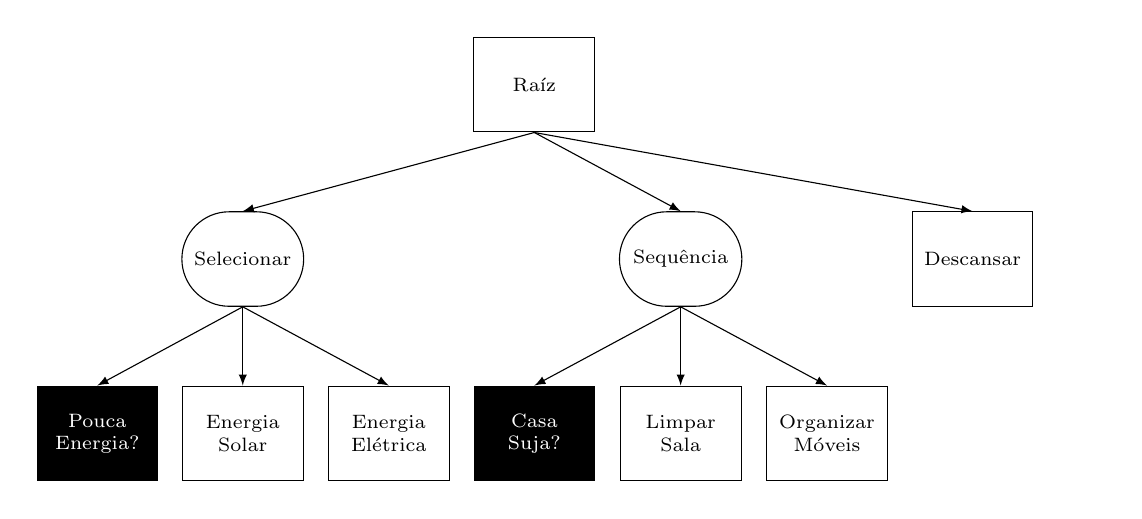
\begin{tikzpicture}[
    every node/.style={
        font=\scriptsize
    },
    composite/.style={
        minimum width=1.3cm, minimum height=1.2cm,
        text width=1.3cm,
        text centered,
        rounded rectangle,
        draw
    },
    action/.style={
        minimum width=1.3cm, minimum height=1.2cm,
        text width=1.3cm,
        text centered,
        rectangle,
        draw
    },
    precond/.style={
        minimum width=1.3cm, minimum height=1.2cm,
        text width=1.3cm,
        text centered,
        rectangle,
        fill=black,
        text=white
    }
]
\matrix [row sep=1cm, column sep=0.3cm] {
                                                &
                                                &
                                                &
    \node (n1)  [action]    {Raíz};             &
                                                &
                                                &
                                                &
                                                &
                                                &
    \\
                                                &
    \node (n2)  [composite] {Selecionar};       &
                                                &
                                                &
    \node (n4)  [composite] {Sequência};        &
                                                &
    \node (n3)  [action]    {Descansar};        &
                                                &
                                                &
    \\
    \node (n5)  [precond]   {Pouca Energia?};   &
    \node (n7)  [action]    {Energia Solar};    &
    \node (n6)  [action]    {Energia Elétrica}; &
    \node (n8)  [precond]   {Casa Suja?};       &
    \node (n9)  [action]    {Limpar Sala};      &
    \node (n10) [action]    {Organizar Móveis}; &
                                                &
                                                &
                                                &
    \\
};
\draw[->,>=latex] (n1.south) -- (n2.north);
\draw[->,>=latex] (n1.south) -- (n3.north);
\draw[->,>=latex] (n1.south) -- (n4.north);

\draw[->,>=latex] (n2.south) -- (n5.north);
\draw[->,>=latex] (n2.south) -- (n6.north);
\draw[->,>=latex] (n2.south) -- (n7.north);

\draw[->,>=latex] (n4.south) -- (n8.north);
\draw[->,>=latex] (n4.south) -- (n9.north);
\draw[->,>=latex] (n4.south) -- (n10.north);
\end{tikzpicture}
\caption {\label{fig:behavior-tree-example}Exemplo de uma \textit{behaviour
tree} para representar um agente que deve carregar suas baterias caso seja
necessário, além de limpar e organizar a casa, descansando caso contrário.}
\end{figure}

Existem algumas outras técnicas que resolvem o mesmo problema que as
\textit{Behavior Trees} como, por exemplo, as \textbf{\textit{Finite State
Machines}} (máquinas de estados finitos), que são muito utilizadas em
inteligência artificial para jogos. Uma \textit{FSM} contém \textbf{estados} que
são ligados através de \textbf{transições}. Contudo, existem diversos problemas
com esta abordagem. A quantidade de estados e transições cresce
exponencialmente, os estados não podem ser reutilizados com facilidade e devemos
nos preocupar constantemente se existem transições inválidas no modelo. As
\textit{FSMs} possuem, resumidamente, um problema de modularidade.

Outra técnica muito utilizada são as \textbf{\textit{Hierarchical Finite State
Machines}} (máquinas de estados finitos hierárquicas). O objetivo da criação
desta técnica foi justamente mitigar alguns dos problemas das \textit{FSMs},
permitindo o englobamento de estados em uma hierarquia. Entretanto, o problema
de extensibilidade e praticidade ainda existem, porque ainda é baseada em
transições.


%----------
\section{\label{section:neat}NEAT}
% NEAT
% neuroevolução
% NEAT evolui os pesos e a rede em sí (TWEANNs)
% representação genética da rede
% problemas comuns em TWEANNs que o NEAT resolve
% (competing conventions, protecting innovation e initial population)

\begin{mdframed}[backgroundcolor=green!20]
\begin{itemize}
    \item
        Introdução: Escolha da técnica, história, paper
    \item
        Relação com aprendizado de máquina
    \item
        Relação com algoritmos genéticos
    \item
        Relação com redes neurais
    \item
        Explicação sobre a técnica: detalhamento de como funciona, termos
        técnicos, exemplos, pedaços de código (se necessário)
    \item
        Como será utilizada na construção dos \textit{bots}
\end{itemize}
\end{mdframed}

\chapter{\label{chap:related-work}Trabalhos Relacionados}
As tarefas de criar uma inteligência artificial para personagens em jogos
digitais e de criar agentes inteligentes capazes de aprender a jogar jogos
digitais já foram exploradas em outros trabalhos. Neste capítulo, selecionamos
três trabalhos que se propuseram a resolver estas tarefas, indicando sua
relevância e similaridade com o projeto presente neste trabalho. 


%----------
\section{Handling Complexity in the Halo 2 AI}
A criação de agentes inteligentes com comportamentos cada vez mais complexos é
uma busca constante para desenvolvedores de jogos digitais. Criar comportamentos
complexos, contudo, vem com um preço -- que muitas vezes o desenvolvedor não
pode pagar --, como a falta de escalabilidade da arquitetura, mais tempo de
processamento ou até mesmo uma experiência ruim de interação entre jogador e
agentes inteligentes.

Este artigo é uma tentativa de elaborar um formalismo de inteligência
artificial, as \textit{Behavior Trees}, para auxiliar na criação de
comportamentos inteligentes para agentes em jogos digitais que sejam de
processamento rápido e ao mesmo tempo sofisticados, fáceis de controlar e
modularizados. As \textit{Behavior Trees} foram utilizadas para desenvolver os
comportamentos dos agentes no jogo \textit{Halo 2}, da desenvolvedora
\textit{Bungie}, e apresentaram resultados muito satisfatórios \cite{Halo2AI}.

Uma \textit{Behavior Tree} é uma estrutura de dados baseado em árvore que
consiste na organização, seleção e execução de \textbf{comportamentos} que o
agente pode executar. Cada comportamento possui uma pré-condição para executar e
uma ação, especificando como o agente atuará para este comportamento. A cada
etapa de execução, o algoritmo examina as pré-condições dos comportamentos e
decide qual comportamento é o mais adequado para executar. Esta técnica está em
rápida ascenção, pois se comparado a máquinas de estados finitos, uma técnica
muito utilizada pela indústria de jogos, são mais modulares e
extensíveis \cite{Rabin:2015:GAP:2821138}.

Esta técnica não é utilizada para criação de agentes inteligentes que jogam
jogos digitais, e sim para criação de comportamentos de agentes. Contudo, não
deixa de ser interessante para este trabalho porque, se comparado a técnicas de
inteligência artificial que envolvem treinamento, permite um controle maior
sobre os comportamentos que a inteligência artificial executa. É possível que,
se adaptada corretamente, o uso desta técnica resulte no sucesso de criação de
\textit{bots}, pois a inteligência artificial, em sua síntese, estaria
executando um comportamento no final das contas.


%----------
\section{Playing Atari with Deep Reinforcement Learning}
O artigo apresenta um modelo de \textit{deep learning} capaz de aprender
políticas de controle para sete jogos do \textit{console} Atari 2600, criando
uma inteligência artificial capaz de jogar eficientemente todos os jogos,
inclusive superando jogadores humanos em alguns
deles \cite{DBLP:journals/corr/MnihKSGAWR13}. O modelo utiliza aprendizado por
reforço e uma rede neural convolucional treinada com uma variante de
\textit{Q-learning} para criar o agente.

Para criar estas políticas de controle, os autores utilizaram uma plataforma de
testes de inteligência artificial chamada \textit{Arcade Learning
Environment}\footnote{http://www.arcadelearningenvironment.org/}.  A cada passo
de execução, o agente interage com o emulador, recebendo informações do estado
do jogo e enviando os comandos que deseja executar. As informações recebidas
eram um vetor dos \textit{pixels} apresentados na tela, o conjunto de de ações
possíveis para o jogo em questão e um valor de recompensa quando a pontuação do
jogo era alterada.

Como as informações do estado do jogo eram altamente dimensionais -- 33600
\textit{pixels} de informação visual --, foi necessário realizar um
pré-processamento para reduzir a dimensionalidade do estado do jogo -- reduzindo
para 7600 \textit{pixels}. Mesmo com esta redução, a quantidade de informações
recebidas ainda era consideravelmente grande. Por isto, a utilização de
\textit{deep learning} e redes neurais convolucionais provou ser uma excelente
-- e necessária -- escolha para realizar o treinamento do agente. Contudo, o
treinamento do agente utilizando esta técnica é extremamente demorado.

Como a dimensionalidade do estado do jogo fornecido pela ferramenta
\textit{SpelunkBots} não é tão grande quanto a do trabalho em questão, optamos
por não fazer uso de \textit{deep learning}, mesmo que a técnica também seja
muito promissora.


%----------
\section{A Neuroevolution Approach to General Atari Game Playing}
Este artigo \cite{NeuroEvolutionAtari} apresenta uma série de abordagens
neuroevolutivas para realizar a criação de agentes inteligentes capazes de
aprender a jogar jogos do \textit{console} \textit{Atari 2600} com pouco
conhecimento específico sobre os domínios dos jogos. Para criar estas políticas
de controle, os autores utilizaram uma plataforma de testes de inteligência
artificial chamada \textit{Arcade Learning Environment}.

Os autores realizaram testes com quatro algoritmos neuroevolutivos, que
descrevem redes neurais artificiais e a evolução de seus componentes:
\textit{Conventional Neuroevolution}, (CNE) \textit{Covariance Matrix Adaptation
Evolution Strategy} (CMA-ES), \textit{Neuroevolution of Augmenting Topologies}
(NEAT) e \textit{Hypercube-based Neuroevolution of Augmenting Topologies}
(HyperNEAT). Os dois primeiros algoritmos evoluem somente os pesos da rede,
enquanto que os dois últimos evoluem os pesos e a topologia da rede. O único
algoritmo que utiliza uma representação genética indireta é o \textit{HyperNEAT}
(os outros representam diretamente).

Os autores optaram por realizar a representação de estados dos jogos de três
maneiras distintas: objetos da tela de jogo, os \textit{pixels} da tela e ruído.
A representação de objetos é a representação de mais alto nível, pois apresenta
uma caracterização informativa e clara da informação visual do jogo. A
representação por \textit{pixels} é uma representação de baixo nível, pois provê
as informações cruas da tela para o agente. É o tipo de representação mais
genérico e o mais fácil de ser aplicado para diversos jogos, e imita as
informações que um jogador humano utilizaria se estivesse jogando.  Foi
necessário realizar um \textit{downsampling}\footnote{Processo de reduzir a taxa
de amostragem de um sinal. Geralmente é aplicado para reduzir a taxa e o tamanho
dos dados recebidos.} dos valores de \textit{pixels} da tela, pois o espaço de
estados era muito grande. A representação por ruído foi utilizada para servir
como base de comparação e investigar quanto do aprendizado é baseado na
memorização e em conceitos gerais.

Após a análise dos dados coletados, os autores identificaram que os algoritmos
neuroevolutivos que utilizam condificação genética direta tendem a obter
melhores resultados quando uma representação compacta de estados (objetos da
tela de jogo) é utilizada, enquanto que os algoritmos neuroevolutivos que
utilizam codificação genética indireta permitem a utilização de uma
representação com maior número de dimensões (como os \textit{pixels} da tela).
Os algoritmos com os melhores resultados, em todas as categorias de
representação de estados, foram o \textit{NEAT} e o \textit{HyperNEAT}.

De acordo com os autores, o uso de neuroevolução ajuda a diminiur os problemas
que as abordagens anteriores de criação de agentes jogadores baseadas em
\textit{Temporal Difference Learning} sofriam, como um grande espaço de estados
e gradientes de recompensa esparsas (ambos encontrados em jogos de
\textit{Atari}). Além disso, as políticas de controle evoluídas através de
algoritmos neuroevolutivos atingem resultados excelentes e, em alguns jogos,
superam o desempenho de jogadores humanos, sugerindo que a neuroevolução é uma
abordagem promissora para criação de agentes inteligentes e \textit{general
video game playing} (criar um agente que seja capaz de jogar diversos jogos
digitais sem mudanças de parâmetros).


%----------
\section{MarI/O}
Em junho de 2015, o canal do \textit{YouTube}
SethBling\footnote{https://www.youtube.com/user/sethbling/about} -- conhecido
por publicar vídeos de modificações de jogos como Mario e Minecraft -- divulgou
o vídeo \textit{MarI/O - Machine Learning for Video
Games}\footnote{https://www.youtube.com/watch?v=qv6UVOQ0F44}, que mostra um
jogador muito habilidoso completando o nível \textit{Donut Plains 1} de
\textit{Super Mario World}. É explicado, então, que o jogador em questão não é
humano, mas sim um programa de computador. Utilizando um emulador de
\textit{consoles} chamado
\textit{BizHawk}\footnote{http://tasvideos.org/BizHawk.html}, a linguagem de
programação \textit{Lua} e uma técnica de inteligência artificial chamada
\textit{\textbf{NEAT}} (\textit{NeuroEvolution of Augmenting Topologies})
\cite{stanley:ec02} -- explicada detalhadamente no capítulo \ref{chap:theory}
--, o autor programou um \textit{bot} capaz de aprender como jogar o nível em
questão do início ao fim com sucesso. Como é explicado no vídeo, inicialmente o
\textit{bot} não conhecia absolutamente nada sobre como jogar \textit{Super
Mario World}. Contudo, através de várias simulações, adquiriu o conhecimento
necessário para superar todos os obstáculos presentes no nível.

\begin{figure}[htb!]
\centering
\includegraphics[width=.65\textwidth]{fig/mar-io-example.pdf}
\caption{\label{fig:mar-io-example}Exemplo da visão do jogo \textit{Super
Mario World} através do projeto \textit{MarI/O}, mostrando elementos de
controle usados pelo NEAT, como a rede neural, as possíveis ações, as
gerações, as espécies, os genomas, entre outros.}
\end{figure}

Depois do sucesso no nível \textit{Donut Plains 1}, o autor realizou mais
experimentos da aplicação da técnica
\textit{NEAT}\footnote{https://www.youtube.com/watch?v=iakFfOmanJU}
\footnote{https://www.youtube.com/watch?v=S9Y\_I9vY8Qw}. Inicialmente, testou em
dois outros níveis de \textit{Super Mario World}. Em \textit{Donut Plains 4}, o
processo de aprendizagem foi complicado, pois para obter progresso no nível era
necessário que aprendesse a interagir com certos elementos do mapa, e o autor
decidiu abortar o processo de aprendizagem. Já em \textit{Yoshi's Island 1},
obteve sucesso e foi capaz de concluir o nível. Com os testes finalizados, o
autor decidiu aplicar a técnica em outros dois jogos da franquia \textit{Mario}.
Em \textit{Super Mario Bros}, o \textit{bot} concluiu o primeiro nível e,
surpreendentemente, foi capaz de descobrir um \textit{glitch} no jogo que o
permitia passar por um segmento do segundo nível com maior rapidez. Em
\textit{Super Mario Kart}, depois de receber treinamento, o \textit{bot} foi
capaz de terminar uma corrida no nível \textit{Mario Circuit 1} em primeiro
lugar contra outros jogadores controlados pelo computador -- na dificuldade mais
fácil do jogo.

O \textit{MarI/O} é especialmente interessante e relevante porque tem um
objetivo muito similar ao deste trabalho: criar uma inteligência artificial
capaz de jogar uma partida de um jogo. Contudo, nos jogos escolhidos por
SethBling, os níveis são sempre os mesmos, o que torna mais fácil medir o
desempenho de um \textit{bot}, pois a disposição do nível é sempre igual e o
objetivo final sempre se encontra no mesmo lugar. Este não é o caso em
\textit{Spelunky}, onde os níveis são gerados proceduralmente. Além disso, os
níveis de \textit{Super Mario World} e \textit{Super Mario Bros.} são
essencialmente horizontais, e movimentar o personagem para a direita quase
sempre garante alguma forma de progresso. Isto facilita ainda mais o processo de
treinamento dos \textit{bots}. Em \textit{Spelunky} não é possível saber de
antemão onde se encontra a saída do nível e o movimento horizontal não garante o
progresso, visto que os níveis não são essencialmente horizontais. Estes fatores
influenciam na dificuldade de realizar o treinamento dos \textit{bots}.

\chapter{\label{chap:project}Projeto}

\todoin[caption={Melhorias para o capítulo}]
{
	\begin{itemize}
		\item O Problema
		\begin{itemize}
			\item Complexidade computacional de jogos
			\item Spelunky não é um platformer tradicional
			\begin{itemize}
				\item Níveis gerados proceduralmente (saída em lugares diferentes)
				\item Navegação horizontal e vertical
				\item Terreno destrutível
			\end{itemize}
			\item Domínio com diversos problemas a serem tratados
				\begin{itemize}
					\item Navegação
					\item Combate
					\item Planejamento e Estratégias
				\end{itemize}
		\end{itemize}

		\item Objetivos
		\begin{itemize}
			\item Detalhar qual problema queremos explorar
			\item Utilizar técnica NEAT para desenvolver os bots
			\item Treinar e testar os bots em cenários de testes pré-determinados
			\item Analisar os resultados obtidos
			\item Comparar com implementações existentes de bots para Spelunky
		\end{itemize}

		\item Técnicas de Inteligência Artificial Utilizadas
		\begin{itemize}
			\item Por que escolhemos NEAT
			\item Falar sobre porque não vamos utilizar Behavior Trees mais
			\item Comparar com outras implementações de bots para Spelunky
		\end{itemize}
	\end{itemize}
}

%----------
\section{\label{section:problem}O Problema}
A prática de estabelecer a complexidade computacional de jogos -- sejam jogos de
carta, jogos de tabuleiro ou jogos digitais -- ajuda a compreender  porque
humanos consideram interessantes os desafios impostos por estes jogos, além de
indicar para pesquisadores da área os desafios propostos vistos de uma
perspectiva de tarefa de otimização.  Dados os desafios presentes em Spelunky
concluiu-se que, computacionalmente falando, trata-se de um problema, no melhor
dos casos, do conjunto \textit{NP-Hard}\cite{SPELUNKYHARD}. O jogo apresenta uma
série de características -- abordadas em detalhe no capítulo \ref{chap:spelunky}
que influenciam fortemente na dificuldade imposta pelo jogo.

Os níveis trazem grandes dificuldades aos jogadores. Em primeiro lugar, o
ambiente em Spelunky é \textbf{contínuo}, \textbf{parcialmente observável},
\textbf{dinâmico}, \textbf{estocástico} e \textbf{sequencial}. Em segundo
lugar, os níveis são gerados proceduralmente, impossibilitanto a memorização do
mapa.  Contudo, o algoritmo utilizado para gerar os níveis garante que existe
pelo menos um caminho transponível do início ao fim -- mesmo que com inimigos e
armadilhas no caminho --, sem que seja necessário o uso de bombas ou cordas
para ajudar na desobstrução do caminho e deslocamento. Sabe-se, também, que o
personagem sempre entra em um nível pela parte superior do mapa, e que a saída
sempre está localizada na parte inferior do mapa. Por fim, cada área em
\textit{Spelunky} possui diferentes características, como tipo de terreno e
monstros diferentes.

Em \textit{Spelunky}, os pontos de vida são o recurso mais importante do
jogador, pois quando esgotados, encerra-se a partida. Existem diversos tipos de
inimigos, armadilhas e perigos naturais cujo único objetivo é impedir o
progresso do jogador.  Somado a isto, depois de 150 segundos em um nível, o
jogador será perseguido incansávelmente por um fantasma que o elimina com apenas
um toque, o que impõe um ''limite`` de tempo que o jogador pode permanecer em um
nível.

O jogo permite que o jogador execute um grande número de ações -- e combinações
de ações -- a cada etapa de atualização do jogo. Algumas delas são influenciadas
por itens equipados ou o estado atual do jogador (no ar, pendurado, etc.), o que
significa que a inteligência artificial desenvolvida deve estar preparada pra
lidar com uma gama gigantesca de possibilidades, pois se não houver cautela, a
execução de uma ação pode gerar resultados inesperados.


%----------
\section{\label{section:objectives}Objetivos}
\todo[inline]{Atualizar objetivos para exploracao de mapa}
Com os desafios e dificuldades apresentados na seção \ref{section:problem}, o
\textbf{objetivo principal} deste trabalho é desenvolver \textit{bots} para o
jogo \textit{Spelunky} que terão como meta se deslocarem do início ao fim de
todos os quatro níveis da área das Minas. Depois da construção dos agentes
inteligentes, coletaremos dados de suas execuções em alguns níveis para realizar
uma análise e comparação aprofundada entre os resultados obtidos por cada
técnica.


%----------
\section{\label{section:techniques}Técnicas de Inteligência Artificial
Utilizadas}
\todo[inline]{Adequar para a saida de Behavior Trees}
Para implementar os \textit{bots} de \textit{Spelunky}, optamos por utilizar as
técnicas \textbf{\textit{NEAT}} e \textbf{\textit{Behavior Trees}}. A
neuroevolução é um modelo de aprendizado de máquina muito utilizado atualmente
para criar agentes jogadores de jogos digitais \cite{DBLP:journals/corr/RisiT14}
e, como vimos no capítulo \ref{chap:related-work}, os resultados obtidos até
agora com este tipo de técnica são muito satisfatórios, muitas vezes superando
as habilidades de jogadores humanos \cite{NeuroEvolutionAtari}. Com isto em
mente, a técnica \textit{NEAT} foi uma escolha natural para este trabalho.

As \textit{Behavior Trees} são muito utilizadas para ajudar na criação de
comportamentos inteligentes para agentes em jogos digitais. Normalmente, esta
técnica não é utilizada para construir agentes jogadores de jogos, mas nada
impede que o formalismo atue neste escopo também. As técnicas de criação de
agentes inteligentes baseadas em aprendizado de máquina são muito poderosas, mas
ao mesmo tempo podem ser vistas como uma ''caixa preta``, pois muitas vezes é
difícil de compreender exatamente o que o agente está pensando e aprendendo.
Optamos por utilizar \textit{Behavior Trees} pois esta técnica permite um ajuste
refinado do comportamento de agentes inteligentes. Assim, esta técnica servirá
de \textbf{base de referência} para medirmos a qualidade dos resultados obtidos
entre uma técnica ''manual`` (\textit{Behavior Trees}) e uma técnica
''automatizada`` (\textit{NEAT}).


\chapter{\label{chap:work-plan}Etapas do Trabalho}

A execução do trabalho particiona-se em iterações de uma semana, onde serão
desenvolvidos uma ou mais atividades. A tabela a seguir ilustra o cronograma
definido para o trabalho, com base nas atividades definidas no capítulo
\ref{chap:objectives}:

\begin{table}[htb!]
\centering
\caption{Objetivos por Iteração}
\label{tab:work-plan}
\begin{tabular}{c|c|c|c|c|c|c|c|c|c|c|c|c|c|c|c|}
\cline{2-16}
{\bf}                                 & \multicolumn{3}{c|}{{\bf Ago/16}} & \multicolumn{4}{c|}{{\bf Set/16}}     & \multicolumn{4}{c|}{{\bf Out/16}}      & \multicolumn{4}{c|}{{\bf Nov/16}}     \\ \hline
\multicolumn{1}{|c|}{{\bf Atividade}} & {\bf 1} & {\bf 2} & {\bf 3}	      & {\bf 4} & {\bf 5} & {\bf 6} & {\bf 7} & {\bf 8} & {\bf 9} & {\bf 10} & \bf{11} & \bf{12} & \bf{13} & \bf{14} & \bf{15} \\ \hline
\multicolumn{1}{|c|}{{\bf 1}}         & X       &         &               &         &         &         &         &         &         &          &         &         &         &         &         \\ \hline
\multicolumn{1}{|c|}{{\bf 2}}         & X       &         &               &         &         &         &         &         &         &          &         &         &         &         &         \\ \hline
\multicolumn{1}{|c|}{{\bf 3}}         &         & X       &               &         &         &         &         &         &         &          &         &         &         &         &         \\ \hline
\multicolumn{1}{|c|}{{\bf 4}}         &         &         & X             &         &         &         &         &         &         &          &         &         &         &         &         \\ \hline
\multicolumn{1}{|c|}{{\bf 5}}         &         &         &               & X       &         &         &         &         &         &          &         &         &         &         &         \\ \hline
\multicolumn{1}{|c|}{{\bf 6}}         &         &         &               &         & X       & X       & X       &         &         &          &         &         &         &         &         \\ \hline
\multicolumn{1}{|c|}{{\bf 7}}         &         &         &               &         &         &         &         & X       &         &          &         &         &         &         &         \\ \hline
\multicolumn{1}{|c|}{{\bf 8}}         &         &         &               &         &         &         &         &         & X       &          &         &         &         &         &         \\ \hline
\multicolumn{1}{|c|}{{\bf 9}}         &         &         &               &         &         &         &         &         &         & X        & X       & X       &         &         &         \\ \hline
\multicolumn{1}{|c|}{{\bf 10}}        &         &         &               &         &         &         &         &         &         &          &         &         & X       &         &         \\ \hline
\multicolumn{1}{|c|}{{\bf 11}}        &         &         &               &         &         &         &         &         &         &          &         &         &         & X       & X       \\ \hline
\end{tabular}
\end{table}

\section{Detalhamento das Atividades}

\begin{enumerate}
    \item
        Obter uma cópia do SpelunkBots
    \begin{description}[leftmargin=!,labelwidth=\widthof{\bfseries Descrição}]
        \item [Descrição]
            Para possibilitar o desenvolvimento desse trabalho, preciamos obter
            uma cópia do projeto SpelunkyBots, permitindo então que façamos o
            desenvolvimento de \textit{bots} utilizando esse \textit{framework}.
        \item [Iterações]
            1
        \item [Período]
            01/08/2016 - 08/08/2016
    \end{description}

    \item
		Realizar modificações no \textit{SpelunkBots} para que possa ser
		executado na plataforma \textit{Linux}
    \begin{description}[leftmargin=!,labelwidth=\widthof{\bfseries Descrição}]
        \item [Descrição]
            O SpelunkBots não possui uma distribuição para Linux. Como vamos
            utilizar um servidor para o treinamento dos \textit{bots},
            precisamos fazer adaptações para que o jogo funcione nessa
            plataforma.
        \item [Iterações]
            1
        \item [Período]
            08/08/2016 - 15/08/2016
    \end{description}

    \item
        Buscar por bibliotecas auxiliares para o uso da técnica \textit{NEAT}
    \begin{description}[leftmargin=!,labelwidth=\widthof{\bfseries Descrição}]
        \item [Descrição]
            O uso de bibliotecas acelera o desenvolvimento da aplicação. Dessa
            forma, devemos buscar uma biblioteca para o uso de \textit{NEAT}.
            Caso encontremos tal biblioteca, é necessário ver se a mesma pode
            ser usada no nosso projeto.
        \item [Iterações]
            2
        \item [Período]
            15/08/2016 - 22/08/2016
    \end{description}

    \item
        Buscar por bibliotecas auxiliares para o uso da técnica
        \textit{Behavior Trees}
    \begin{description}[leftmargin=!,labelwidth=\widthof{\bfseries Descrição}]
        \item [Descrição]
            O uso de bibliotecas acelera o desenvolvimento da aplicação. Dessa
            forma, devemos buscar uma biblioteca para o uso de \textit{behavior
            trees}.  Caso encontremos tal biblioteca, é necessário ver se a
            mesma pode
            ser usada no nosso projeto.
        \item [Iterações]
            3
        \item [Período]
            22/08/2016 - 05/09/2016
    \end{description}

	\item
		Realizar as configurações da ferramenta \textit{SpelunkBots} para
		permitir o desenvolvimento de \textit{bots} utilizando \textit{Behavior
		Trees}
    \begin{description}[leftmargin=!,labelwidth=\widthof{\bfseries Descrição}]
        \item [Descrição]
            Devemos estudar como utilizar as bibliotecas de \textit{Behavior
            Trees} encontradas para integrá-las ao código do
            \textit{SpelunkBots}, modificando ou incrementando o código
            existente.
        \item [Iterações]
            4
        \item [Período]
            05/09/2016 - 12/09/2016
    \end{description}
	\item
		Desenvolver um \textit{bot} utilizando \textit{Behavior Trees}
    \begin{description}[leftmargin=!,labelwidth=\widthof{\bfseries Descrição}]
        \item [Descrição]
            Desenvolvimento do código do \textit{bot} que fará uso da técnica
            \textit{Behavior Trees}.
        \item [Iterações]
            5, 6 e 7
        \item [Período]
            12/09/2016 - 03/10/2016
    \end{description}
	\item
		Coletar dados da execução do \textit{bot} baseado em \textit{Behavior
		Trees} em uma série de mapas pré-estabelecidos e aleatórios
    \begin{description}[leftmargin=!,labelwidth=\widthof{\bfseries Descrição}]
        \item [Descrição]
            Coletar dados de execução, exportando os resultados obtidos,
            permitindo que sejam feitas análises sobre o \textit{bot}
            utilizando esses dados.
        \item [Iterações]
            8
        \item [Período]
            03/10/2016 - 10/10/2016
    \end{description}
	\item
		Realizar as configurações da ferramenta \textit{SpelunkBots} para
		permitir o desenvolvimento de \textit{bots} utilizando \textit{NEAT}
    \begin{description}[leftmargin=!,labelwidth=\widthof{\bfseries Descrição}]
        \item [Descrição]
            Devemos estudar como utilizar as bibliotecas de textit{NEAT}
            encontradas para integrá-las ao código do \textit{SpelunkBots},
            modificando ou incrementando o código existente.
        \item [Iterações]
            9
        \item [Período]
            10/10/2016 - 17/10/2016
    \end{description}
	\item
		Desenvolver um \textit{bot} utilizando \textit{NEAT}
    \begin{description}[leftmargin=!,labelwidth=\widthof{\bfseries Descrição}]
        \item [Descrição]
            Desenvolvimento do código do \textit{bot} que fará uso da técnica
            \textit{NEAT}.
        \item [Iterações]
            10, 11 e 12
        \item [Período]
            17/10/2016 - 07/11/2016
    \end{description}
	\item
		Coletar dados da execução do \textit{bot} baseado em \textit{NEAT} em
		uma série de mapas pré-estabelecidos e aleatórios
    \begin{description}[leftmargin=!,labelwidth=\widthof{\bfseries Descrição}]
        \item [Descrição]
            Coletar dados de execução, exportando os resultados obtidos,
            permitindo que sejam feitas análises sobre o \textit{bot}
            utilizando esses dados.
        \item [Iterações]
            13
        \item [Período]
            07/11/2016 - 14/11/2016
    \end{description}
	\item
		Analisar e comparar os resultados obtidos entre os \textit{bots}
		baseados em \textit{Behavior Trees} e \textit{NEAT}
    \begin{description}[leftmargin=!,labelwidth=\widthof{\bfseries Descrição}]
        \item [Descrição]
            Devemos analisar o uso das técnicas escolhidas nesse trabalho,
            verificando o desempenho delas para a solução do problema.
        \item [Iterações]
            14 e 15
        \item [Período]
            14/11/2016 - 28/11/2016
    \end{description}
\end{enumerate}


\appendix
\chapter{\label{appendix:spelunkbots-variables}Lista de Variáveis Globais
de SpelunkBots}

\section{Movimentação do \textit{Bot}}

\begin{center}
    \begin{tabular}{ |c| }
        \hline
        \textbf{Variável} \\ \hline
        global.attack \\ \hline
        global.duck \\ \hline
        global.goLeft \\ \hline
        global.goRight \\ \hline
        global.jump \\ \hline
        global.lookUp \\ \hline
        global.payp \\ \hline
        global.running \\ \hline
    \end{tabular}
\end{center}

\section{Tipo do Terreno}

\begin{center}
    \begin{tabular}{ |c|c| }
        \hline
        \textbf{Variável} & \textbf{Valor} \\ \hline
        global.spEmptyNode & 0 \\ \hline
        global.spStandardTerrain & 1 \\ \hline
        global.spLadder & 2 \\ \hline
        global.spEntrance & 3 \\ \hline
        global.spExit & 4 \\ \hline
        global.spSacAlter & 5 \\ \hline
        global.spArrowTrapRight & 6 \\ \hline
        global.spArrowTrapLeft & 7 \\ \hline
        global.spIsInShop & 8 \\ \hline
        global.spIce & 9 \\ \hline
        global.spSpike & 10 \\ \hline
        global.spSpearTrap & 11 \\ \hline
    \end{tabular}
\end{center}

\section{Inimigos e Armadilhas}

\begin{center}
    \begin{tabular}{ |c|c| }
        \hline
        \textbf{Variável} & \textbf{Valor} \\ \hline
        global.spGhost & 1 \\ \hline
        global.spBat & 2 \\ \hline
        global.spScarab & 3 \\ \hline
        global.spSpider & 4 \\ \hline
        global.spGiantSpiderHang & 5 \\ \hline
        global.spGiantSpider & 6 \\ \hline
        global.spFrog & 7 \\ \hline
        global.spFireFrog & 8 \\ \hline
        global.spZombie & 9 \\ \hline
        global.spVampire & 10 \\ \hline
        global.spPiranha & 11 \\ \hline
        global.spJaws & 12 \\ \hline
        global.spDeadFish & 13 \\ \hline
        global.spManTrap & 14 \\ \hline
        global.spMonkey & 15 \\ \hline
        global.spYeti & 16 \\ \hline
        global.spYetiKing & 17 \\ \hline
        global.spUFO & 18 \\ \hline
        global.spUFOCrash & 19 \\ \hline
        global.spAlienEject & 20 \\ \hline
        global.spAlien & 21 \\ \hline
        global.spAlienBoss & 22 \\ \hline
        global.spBarrierEmitter & 23 \\ \hline
        global.spBarrier & 24 \\ \hline
        global.spCaveman & 25 \\ \hline
        global.spHawkman & 26 \\ \hline
        global.spMagma & 27 \\ \hline
        global.spMagmaTrail & 28 \\ \hline
        global.spMagmaMan & 29 \\ \hline
        global.spTombLord & 30 \\ \hline
    \end{tabular}
\end{center}

\begin{center}
    \begin{tabular}{ |c|c| }
        \hline
        global.spOlmec & 31 \\ \hline
        global.spCavemanWorship & 32 \\ \hline
        global.spHawkmanWorship & 33 \\ \hline
        global.spOlmecDebris & 34 \\ \hline
        global.spSnake & 35 \\ \hline
        global.spSpiderHang & 36 \\ \hline
        global.spMagmaMan & 37 \\ \hline
        global.spShopkeeper & 38 \\ \hline
        global.spBones & 60 \\ \hline
        global.spSmashTrap & 61 \\ \hline
        global.spCeilingTrap & 62 \\ \hline
        global.spBoulder & 63 \\ \hline
        global.spSpringTrap & 99 \\ \hline
    \end{tabular}
\end{center}

\section{Objetos}

\begin{center}
    \begin{tabular}{ |c|c| }
        \hline
        \textbf{Variável} & \textbf{Valor} \\ \hline
        global.spGoldBar & 1 \\ \hline
        global.spGoldBars & 2 \\ \hline
        global.spEmerald & 3 \\ \hline
        global.spEmeraldBig & 4 \\ \hline
        global.spSapphire & 5 \\ \hline
        global.spSapphireBig & 6 \\ \hline
        global.spRuby & 7 \\ \hline
        global.spRubyBig & 8 \\ \hline
        global.spDiamond & 9 \\ \hline
        global.spGoldNugget & 10 \\ \hline
        global.spGoldChunk & 11 \\ \hline
        global.spChest & 12 \\ \hline
        global.spLockedChest & 13 \\ \hline
        global.spKey & 14 \\ \hline
        global.spCrate & 15 \\ \hline
        global.spFlareCrate & 16 \\ \hline
        global.spBombBag & 17 \\ \hline
        global.spBombBox & 18 \\ \hline
        global.spPaste & 19 \\ \hline
        global.spRopePile & 20 \\ \hline
        global.spParachute & 21 \\ \hline
        global.spCompass & 22 \\ \hline
        global.spSpringShoes & 23 \\ \hline
        global.spSpikeShoes & 24 \\ \hline
        global.spJordans & 25 \\ \hline
        global.spSpecs & 26 \\ \hline
        global.spUdjat & 27 \\ \hline
        global.spCrown & 28 \\ \hline
        global.spKapala & 29 \\ \hline
        global.spAnkh & 30 \\ \hline
        global.spGloves & 31 \\ \hline
        global.spMitt & 32 \\ \hline
        global.spJetpack & 33 \\ \hline
        global.spCape & 34 \\ \hline
        global.spRopeBag & 35 \\ \hline
    \end{tabular}
\end{center}

\section{Dados do Jogador}

\begin{center}
    \begin{tabular}{ |c| }
        \hline
        \textbf{Variável (boolean)} \\ \hline
        global.hasGoal \\ \hline
        global.spIsInAir \\ \hline
        global.spIsJetpacking \\ \hline
        global.spJumpPressedPreviously \\ \hline
        global.itemGoal \\ \hline
        global.fogGoal \\ \hline
        global.endGoal \\ \hline
        global.headingRight \\ \hline
        global.headingLeft \\ \hline
        global.isPlayerHanging \\ \hline
        global.isPlayerHodldingHoldenIdol \\ \hline
    \end{tabular}
\end{center}

\begin{center}
    \begin{tabular}{ |c| }
        \hline
        \textbf{Variável (número inteiro)} \\ \hline
        global.playerPositionX \\ \hline
        global.playerPositionY \\ \hline
        global.playerPositionXNode \\ \hline
        global.playerPositionYNode \\ \hline
        global.pathCount \\ \hline
        global.tempID \\ \hline
        global.waitTimer \\ \hline
    \end{tabular}
\end{center}

\chapter{\label{appendix:spelunkbots-algorithms}Algoritmos Básicos Para
Implementação de \textit{Bots} Utilizando \textit{SpelunkBots}}

\section{Arquivo de \textit{Header}}

\begin{algorithm}[H]
\lstinputlisting[style=customC++]{code/ExampleBot.h}
\caption[Definição de métodos e variáveis de um \textit{bot} de exemplo.]
{\label{alg:project-example-bot-header}Definição de métodos e variáveis de um
\textit{bot} de exemplo.}
\end{algorithm}

\section{Implementação dos Métodos e Variáveis}

\begin{algorithm}[H]
\lstinputlisting[style=customC++]{code/ExampleBot.cpp}
\caption[Implementação dos métodos e variáveis de um \textit{bot} de exemplo.]
{\label{alg:project-example-bot-impl}Implementação dos métodos e variáveis de um
\textit{bot} de exemplo.}
\end{algorithm}


\bibliographystyle{tcc-num}
\bibliography{final-assignment-1-bib}

\end{document}
